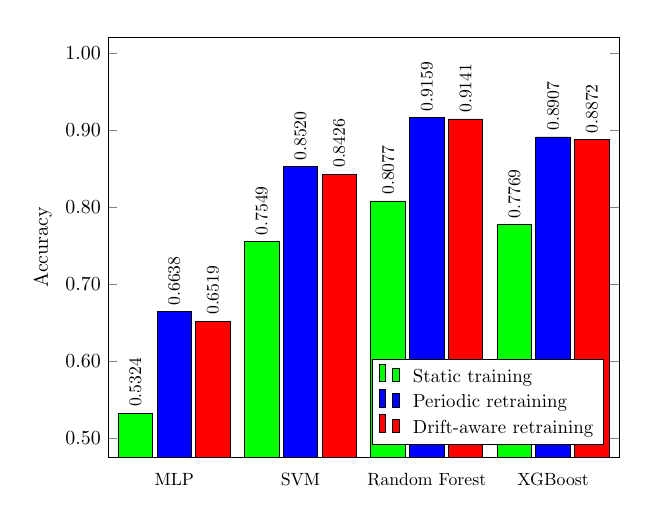
\begin{tikzpicture}[scale=0.8, every node/.style={scale=1.0}]
\pgfkeys{/pgf/number format/.cd,1000 sep={}}
\begin{axis}[%axis x line*=bottom,
	%bar shift=0pt,
        width  = 0.8*\textwidth,
        height = 8.25cm,
        ymin=0.475,ymax=1.02,
%        ytick={0.0, 0.1, 0.2, 0.3, 0.4, 0.5, 0.6, 0.7, 0.8, 0.9, 1.0},
        ytick={0.50, 0.60, 0.70, 0.80, 0.90, 1.00},
        major x tick style = transparent,
        ybar=5*\pgflinewidth,
%        bar width=15.0pt,
        bar width=15.5pt,
%        ymajorgrids = true,
%        xlabel = {Learning technique},
        ylabel = {Accuracy},
        ylabel style = {scale = 0.9},
%        symbolic x coords={A,B,C,D},
%        xticklabels={SVC, Random Forest, MLP, XGBoost},
        symbolic x coords={C, A, B, D},
        xticklabels={MLP,  SVM, Random Forest, XGBoost},
 	y tick label style={scale=0.9,
%		rotate=60,
    		/pgf/number format/.cd,
   		fixed,
   		fixed zerofill,
%		sep=,
    		precision=2},
%	yticklabel pos=right,
        xtick = data,
        x tick label style={scale=0.8,
%        		rotate=60,
%%		font=\small,
%		anchor=north east,
%		inner sep=0mm
		},
%		font=\small},
%        scaled y ticks = false,
	%%%%% numbers on bars and rotated
        nodes near coords,
        every node near coord/.append style={rotate=90, scale=0.8,
        								   anchor=west, 
								   %font=\footnotesize,
								   /pgf/number format/.cd,
								   fixed,
								   fixed zerofill,
%								   sep=,
								   precision=4},
        %%%%%
%        enlarge x limits=0.03,
%        enlarge x limits=0.06,
        enlarge x limits=0.175,
        legend cell align=left,
        legend pos=south east,
        legend style={nodes={scale=0.85},
%%                at={(1,1.05)},
%%                anchor=south east,
%%	        nodes={rotate=90},%%%%% rotate text in legend
%%                at={(0.125,0)},
%%                at={(0.125,0)},
%%                at={(0.8775,0)},
%                at={(0.80,0.01)},
%                at={(0.80,0.25)},
%                anchor=south,
                column sep=1ex
        },
]
\addplot [fill=green,opacity=1.00]
coordinates {
(C,0.5324)
(A,0.7549)
(B,0.8077)
(D,0.7769)
};
\addlegendentry{Static training}
\addplot [fill=blue,opacity=1.00]
coordinates {
(C,0.6638)
(A,0.8520)
(B,0.9159)
(D,0.8907)
};
\addlegendentry{Periodic retraining}
\addplot [fill=red,opacity=1.00]
coordinates {
(C,0.6519)
(A,0.8426)
(B,0.9141)
(D,0.8872)
};
\addlegendentry{Drift-aware retraining}
\end{axis}
\end{tikzpicture}
